\chapter{Uncertainty, Time Evolution, and Spin Precession}

Tonight's lecture follows a very characteristic arc. We begin with uncertainty, but not yet with a quantitative inequality. Instead we begin with the simpler and deeper question: when can two observables be sharp together? From there we return to the general machinery of time evolution, identify the Hamiltonian as the Hermitian generator of that evolution, solve the Schr\"odinger equation in the energy basis, and only then cash out the formalism on the simplest truly quantum example, a single spin in a magnetic field. What follows is a companion rendering of Leonard Susskind's lecture, with the board record preserved through the curation of LazyingArt LLC and Video2Book.

\begin{figure}[ht]
\centering

\includegraphics[width=0.72\textwidth]{lecture_05_figure_01.png}
\caption{Stanford University opening card.}
\end{figure}

\section{Simultaneous Measurement, Common Eigenvectors, and Commutativity}

We begin with a good measurement. A good measurement is not merely one that produces a number; it is one that leaves the system, at least momentarily, in a state for which that number is definite. In the present language, that means the system is left in an eigenvector of the corresponding observable operator.

\begin{definition}
An observable is represented by a Hermitian operator. Its possible measurement outcomes are its eigenvalues, and a state in which that observable is definite is an eigenvector of that operator.
\end{definition}

Suppose now that two observables can be simultaneously measured. Then a successful simultaneous measurement must leave the system in a state that is definite for both observables. That is the whole conceptual engine of the argument.

\begin{remark}
Throughout this lecture Susskind uses the word \emph{basis} in the physicist's sense: a complete orthonormal basis. He pauses to note that mathematicians allow a more general notion, but orthonormality is the relevant notion here.
\end{remark}

\begin{theorem}
If two observables can be simultaneously measured, then the corresponding Hermitian operators commute.
\end{theorem}

\begin{figure}[ht]
\centering

\includegraphics[width=0.82\textwidth]{lecture_05_figure_02.png}
\caption{\(ML\) and \(LM\) acting the same on the basis.}
\end{figure}

\begin{proof}
Let \(L\) and \(M\) be the two observables. Simultaneous measurability means that there is a complete orthonormal basis \(\{|i\rangle\}\) consisting of simultaneous eigenvectors:
\begin{equation}
L|i\rangle = l_i |i\rangle,
\qquad
M|i\rangle = m_i |i\rangle.
\end{equation}
Now act with the two operators in the two possible orders:
\begin{align}
ML|i\rangle
&= M(l_i|i\rangle)
 = l_i\,M|i\rangle
 = l_i m_i |i\rangle, \\
LM|i\rangle
&= L(m_i|i\rangle)
 = m_i\,L|i\rangle
 = m_i l_i |i\rangle
 = l_i m_i |i\rangle.
\end{align}
Thus \(ML\) and \(LM\) have the same action on every basis vector. Since any vector is a superposition of basis vectors, \(ML\) and \(LM\) have the same action on every vector. Therefore
\begin{equation}
[L,M] \equiv LM - ML = 0.
\end{equation}
\end{proof}

The lecture also states the converse: if two Hermitian operators commute, then one can find a complete basis of simultaneous eigenvectors. That direction is not reproved on the board here, but it is part of the standard theorem. For present purposes, the point is that simultaneous measurability and commutativity go together.

This immediately illuminates the spin operators \(\sigma_x,\sigma_y,\sigma_z\). No two of them commute, and therefore no two of them can be simultaneously sharp. The eigenvectors of \(\sigma_z\) are the up and down states; the eigenvectors of \(\sigma_x\) are left and right; they are not the same states, and so the obstruction is already sitting in front of us. That is the qualitative core of uncertainty.

\subsection{Question \& Answer}

\paragraph{Why must simultaneous measurements leave a common eigenbasis?}
The lecturer is asked to slow this point down, and it is worth doing so. If we measure one observable and obtain a value, the system must be left in a state of definite value for that observable; otherwise the measurement would not be repeatable even in principle. If we can measure two observables simultaneously and obtain definite values for both, then the post-measurement state must be definite for both. In other words, it must be an eigenvector of both operators. If this can be done for every possible outcome, we are led to a complete basis of simultaneous eigenvectors.

For a pair such as \(\sigma_x\) and \(\sigma_z\), this fails. Each operator separately may be measured, and each measurement separately may be repeated consistently, but the two kinds of definiteness are incompatible with one another. That is why uncertainty appears before any inequality is written down.

\section{Time Evolution and the Emergence of the Hamiltonian}

Having cleared that conceptual ground, the lecture turns back to time evolution. Susskind explicitly presents this as review, but it is review with a purpose: once we know what a state is, the next task is to understand how it moves.

If the state at time \(0\) is \(|\psi(0)\rangle\), then the state at time \(t\) is obtained by a linear operator \(U(t)\):
\begin{equation}
|\psi(t)\rangle = U(t)|\psi(0)\rangle.
\end{equation}
The key dynamical principle is conservation of distinctions: orthogonal states remain orthogonal. If \(|i\rangle\) and \(|j\rangle\) are orthonormal basis vectors, then after evolution their inner product is unchanged. This implies
\begin{equation}
U^\dagger U = I.
\end{equation}
Thus the time-evolution operator is unitary.

For an infinitesimal time step \(\epsilon\), continuity requires that \(U(\epsilon)\) be close to the identity. We therefore write
\begin{equation}
U(\epsilon) = I - i\epsilon H,
\qquad
U^\dagger(\epsilon) = I + i\epsilon H^\dagger.
\end{equation}
Substituting these into \(U^\dagger U = I\) and keeping only first-order terms in \(\epsilon\), we obtain
\begin{equation}
H^\dagger = H.
\end{equation}
That is big news. The generator of time evolution is Hermitian, and therefore it is an observable. This is the quantum Hamiltonian.

\begin{figure}[ht]
\centering

\includegraphics[width=0.82\textwidth]{lecture_05_figure_03.png}
\caption{Difference quotient for state evolution.}
\end{figure}

Applying \(U(\epsilon)\) to the state and rearranging gives the visible board equation
\begin{equation}
\frac{|\psi(\epsilon)\rangle - |\psi(0)\rangle}{\epsilon} = -iH|\psi(0)\rangle.
\end{equation}
The left-hand side is a difference quotient, so in the limit \(\epsilon \to 0\) we arrive at the time-dependent Schr\"odinger equation,
\begin{equation}
\frac{d}{dt}|\psi\rangle = -iH|\psi\rangle.
\end{equation}

This evolution law has the flavor of determinism, but only of a particular kind. The state vector evolves in a definite way, but the state vector does not encode the answers to all measurements. It encodes probabilities. So the Schr\"odinger equation is best thought of as an update rule for the probability structure carried by the state.

There is also an important qualification. This is the evolution of an undisturbed system. If we measure the system, we generally disturb it. The one easy exception is the special case in which the system was already in an eigenstate of the observable being measured.

\section{Energy Eigenstates and the General Solution of Schr\"odinger Evolution}

Once \(H\) is recognized as an observable, we may ask for its eigenvalues. This is the time-independent Schr\"odinger equation:
\begin{equation}
H|E_i\rangle = E_i |E_i\rangle.
\end{equation}
The possible outcomes of an energy measurement are the eigenvalues \(E_i\). Their detailed values depend on the system: for some systems they form a discrete set, for others a continuous family. But the mathematical task is always the same: diagonalize the Hamiltonian.

\begin{figure}[ht]
\centering

\includegraphics[width=0.82\textwidth]{lecture_05_figure_05.png}
\caption{State expanded in energy eigenvectors.}
\end{figure}

The lecture then returns to a completely general state and expands it in the energy basis. On the board one sees the identification \(|i\rangle = |E_i\rangle\), and the lower line is partly obscured, but the intended expansion is clear:
\begin{equation}
|\psi(t)\rangle = \sum_j \alpha_j(t)\,|j\rangle,
\qquad
|j\rangle \equiv |E_j\rangle.
\end{equation}
The basis vectors are fixed; all the time dependence lives in the coefficients \(\alpha_j(t)\).

Now differentiate:
\begin{equation}
\frac{d}{dt}|\psi(t)\rangle = \sum_j \dot{\alpha}_j(t)\,|j\rangle.
\end{equation}
On the other hand, Schr\"odinger's equation gives
\begin{equation}
-iH|\psi(t)\rangle
=
-i\sum_j \alpha_j(t)\,H|j\rangle
=
-i\sum_j E_j\alpha_j(t)\,|j\rangle.
\end{equation}
Because the same basis vectors appear on both sides, the coefficients must match:
\begin{equation}
\dot{\alpha}_j(t) = -iE_j \alpha_j(t).
\end{equation}
This is a simple first-order differential equation, and its solution is
\begin{equation}
\alpha_j(t) = \alpha_j(0)e^{-iE_j t}.
\end{equation}
Therefore the full state evolves as
\begin{equation}
|\psi(t)\rangle = \sum_j \alpha_j(0)e^{-iE_j t}|j\rangle.
\end{equation}

If we restore \(\hbar\), the phase factor becomes \(e^{-iE_j t/\hbar}\). This is the lecture's first strong link between energy and oscillation. The amplitudes do not change in magnitude; only their relative phases wind in time. That is why the time evolution of a quantum state so often appears as interference.

\section{Expectation Values, Commutators, and the Classical Analogy}

With the general solution in hand, the lecture asks a different question. Instead of following the ket vector itself, how do the average values of observables change?

For a generic observable \(L\), the expectation value is
\begin{equation}
\langle L\rangle = \langle \psi|L|\psi\rangle.
\end{equation}
Differentiate with respect to time. There are two terms, one from the ket and one from the bra. Using the Schr\"odinger equation on the ket and its complex conjugate on the bra, the two terms combine into a commutator.

\begin{figure}[ht]
\centering

\includegraphics[width=0.82\textwidth]{lecture_05_figure_04.png}
\caption{Expectation values evolve by a commutator.}
\end{figure}

The result is the Heisenberg equation in the form used in this lecture:
\begin{equation}
\frac{d}{dt}\langle L\rangle = -i\langle [L,H]\rangle.
\end{equation}
Susskind sometimes writes this more compactly as
\begin{equation}
\dot L = -i[L,H],
\end{equation}
but at this stage that shorthand should still be read under expectation values. The lecture has not yet shifted to a full operator-valued Heisenberg picture.

Using the energy-basis solution, we can also write the expectation value in matrix form:
\begin{equation}
\langle L\rangle(t)
=
\sum_{k,j}\alpha_k^*(0)\alpha_j(0)
e^{i(E_k-E_j)t}
L_{kj},
\qquad
L_{kj}=\langle k|L|j\rangle.
\end{equation}
This is the formula the lecture associates with the matrix point of view: every matrix element carries a frequency difference \(E_k-E_j\).

\subsection{Question \& Answer}

\paragraph{Why does the factor \(i\) not make the time derivative imaginary?}
The lecture raises this objection exactly where it ought to arise. If \(\langle L\rangle\) is real, how can its time derivative equal \(-i\) times something? Susskind does not answer this abstractly first; he promises to answer it by example. The answer is that the commutators of the Hermitian operators we care about come with explicit factors of \(i\). When the spin example is worked out, the unwanted imaginary unit disappears from the final equations of motion for the averages.

Before going to spin, the lecture pauses over the algebra of commutators. First, commutators are odd:
\begin{equation}
[A,B] = -[B,A].
\end{equation}
Second, they satisfy the same product rule as the Poisson bracket:
\begin{proposition}
For operators \(A\), \(B\), and \(C\),
\begin{equation}
[AB,C] = A[B,C] + [A,C]B.
\end{equation}
\end{proposition}

\begin{proof}
We write
\begin{align}
[AB,C]
&= ABC - CAB \\
&= ABC - ACB + ACB - CAB \\
&= A(BC-CB) + (AC-CA)B \\
&= A[B,C] + [A,C]B.
\end{align}
\end{proof}

This is not an accident. Quantum mechanics is more fundamental than classical mechanics, and classical Poisson brackets are best understood as the classical shadow of quantum commutators. In the units used throughout most of the lecture, \(\hbar=1\), and then the structural correspondence is
\begin{equation}
\{L,H\} \longleftrightarrow -i[L,H].
\end{equation}
With \(\hbar\) restored, one writes more carefully
\begin{equation}
\{L,H\} \longleftrightarrow -\frac{i}{\hbar}[L,H].
\end{equation}
That is the reason \(H\) deserves to be called the Hamiltonian.

As an immediate application, set \(L=H\). Then
\begin{equation}
\frac{d}{dt}\langle H\rangle = -i\langle [H,H]\rangle = 0.
\end{equation}
So the average energy is conserved.

\section{A Single Spin in a Magnetic Field}

Only now does the lecture finally return to the favorite little system of one spin. The strategy is exactly as promised: take the general formalism, and put it to work.

\begin{figure}[ht]
\centering

\includegraphics[width=0.86\textwidth]{lecture_05_figure_06.png}
\caption{Magnetic field along \(z\) and spin Hamiltonian setup.}
\end{figure}

\begin{figure}[ht]
\centering
\begin{tikzpicture}[scale=1.15]
\draw[->] (0,0) -- (0,2.6) node[above] {$B_z$};
\draw[->] (0.25,0.25) -- (1.65,1.55);
\draw (3.2,1.3) node {$H=\dfrac{\omega}{2}\sigma_z$};
\end{tikzpicture}
\caption{A minimal redraw of the board sketch: a magnetic field along the \(z\)-axis and a tilted spin direction drawn only as a mnemonic.}
\end{figure}

A classical magnetic dipole in a magnetic field has an energy proportional to the dot product of the dipole with the field. The lecture takes the quantum analog as a guess or postulate: if the magnetic field is along the \(z\)-axis, then the Hamiltonian should be proportional to the \(z\)-component of spin. The convenient normalization is
\begin{equation}
H=\frac{\omega}{2}\sigma_z.
\end{equation}
The factor \(\omega/2\) absorbs the magnetic field strength, the magnetic moment, and the relevant constants. The point is not to derive the constant here, but to see what such a Hamiltonian does.

The board sketch is deliberately classical-looking, but the lecture warns us not to take it too literally. A spin is not really a little arrow in space. What we can meaningfully track are expectation values.

We therefore ask for the time derivatives of the spin components:
\begin{align}
\frac{d}{dt}\langle \sigma_x\rangle
&=
-i\left\langle \left[\sigma_x,\frac{\omega}{2}\sigma_z\right]\right\rangle, \\
\frac{d}{dt}\langle \sigma_y\rangle
&=
-i\left\langle \left[\sigma_y,\frac{\omega}{2}\sigma_z\right]\right\rangle, \\
\frac{d}{dt}\langle \sigma_z\rangle
&=
-i\left\langle \left[\sigma_z,\frac{\omega}{2}\sigma_z\right]\right\rangle.
\end{align}
The last of these is immediate:
\begin{equation}
\frac{d}{dt}\langle \sigma_z\rangle = 0.
\end{equation}
So the component of spin along the magnetic field is conserved.

To go further we need the Pauli commutators. The lecture works them out by direct matrix multiplication. For example,
\begin{equation}
[\sigma_z,\sigma_x]
=
\begin{pmatrix}
1&0\\
0&-1
\end{pmatrix}
\begin{pmatrix}
0&1\\
1&0
\end{pmatrix}
-
\begin{pmatrix}
0&1\\
1&0
\end{pmatrix}
\begin{pmatrix}
1&0\\
0&-1
\end{pmatrix}
=
2i\sigma_y.
\end{equation}
Cyclic permutation gives the rest:
\begin{equation}
[\sigma_z,\sigma_x]=2i\sigma_y,
\qquad
[\sigma_x,\sigma_y]=2i\sigma_z,
\qquad
[\sigma_y,\sigma_z]=2i\sigma_x.
\end{equation}
Now the promised resolution of the earlier puzzle arrives explicitly. Since
\begin{equation}
[\sigma_x,\sigma_z]=-2i\sigma_y,
\end{equation}
we find
\begin{align}
\frac{d}{dt}\langle \sigma_x\rangle
&=
-i\frac{\omega}{2}\langle[\sigma_x,\sigma_z]\rangle
=
-i\frac{\omega}{2}\langle -2i\sigma_y\rangle
=
-\omega \langle \sigma_y\rangle,\\
\frac{d}{dt}\langle \sigma_y\rangle
&=
-i\frac{\omega}{2}\langle[\sigma_y,\sigma_z]\rangle
=
-i\frac{\omega}{2}\langle 2i\sigma_x\rangle
=
+\omega \langle \sigma_x\rangle.
\end{align}
Together with \(\dot{\langle \sigma_z\rangle}=0\), these are the equations of circular motion.

\begin{figure}[ht]
\centering
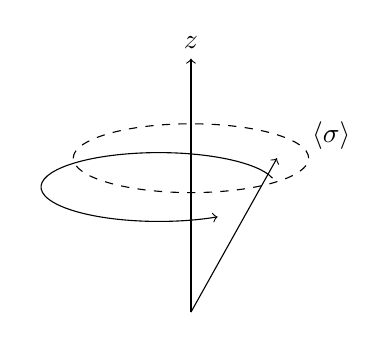
\begin{tikzpicture}[scale=1.15]
\draw[->] (0,0) -- (0,2.8) node[above] {$z$};
\draw[dashed] (0,1.7) ellipse (1.3 and 0.38);
\draw[->] (0,0) -- (0.95,1.7);
\draw[->] (0.9,1.48) arc[start angle=15,end angle=300,x radius=1.3,y radius=0.38];
\draw (1.55,1.95) node {$\langle \sigma \rangle$};
\end{tikzpicture}
\caption{In the sense of expectation values, the spin precesses about the magnetic-field axis.}
\end{figure}

This is the payoff: the expectation values of the spin components precess exactly as a classical rotor or gyroscope precesses in a magnetic field. The lecture is careful here. The operators themselves do not literally move in space. What moves is the pattern of expectation values, because the state changes with time.

\section{General Field Direction and Final Clarifications}

The \(z\)-axis was chosen only for convenience. In fact, for a single spin there are very few Hamiltonians available. The most general Hermitian operator on a two-dimensional state space has the form
\begin{equation}
H = aI + b_x\sigma_x + b_y\sigma_y + b_z\sigma_z.
\end{equation}
The identity term is dynamically uninteresting, since it commutes with everything and merely shifts the zero of energy. So the nontrivial part is a linear combination of the three Pauli matrices. That is exactly what one would expect from coupling a spin to a magnetic field.

If \(\mathbf{B}\) points along a unit vector \(\mathbf{n}\), so that \(\mathbf{B}=B\,\mathbf{n}\), then the natural Hamiltonian is
\begin{equation}
H = \frac{\omega}{2}\,\sigma\cdot n,
\qquad
\sigma\cdot n \equiv n_x\sigma_x + n_y\sigma_y + n_z\sigma_z.
\end{equation}
In matrix form,
\begin{equation}
\sigma\cdot n
=
\begin{pmatrix}
n_z & n_x - i n_y \\
n_x + i n_y & -n_z
\end{pmatrix}.
\end{equation}
If \(n\) is a unit vector, then
\begin{equation}
n_x^2+n_y^2+n_z^2=1.
\end{equation}
The trace of this matrix vanishes,
\begin{equation}
\operatorname{tr}(\sigma\cdot n)=0,
\end{equation}
so the two eigenvalues are equal and opposite. Its determinant is
\begin{equation}
\det(\sigma\cdot n)=-(n_x^2+n_y^2+n_z^2)=-1,
\end{equation}
so the product of the eigenvalues is \(-1\). Therefore the eigenvalues must be
\begin{equation}
\lambda_\pm = \pm 1.
\end{equation}
It follows that the two energy levels are always
\begin{equation}
E_\pm = \pm \frac{\omega}{2},
\end{equation}
and so the energy gap is
\begin{equation}
\Delta E = \omega.
\end{equation}
This is independent of the direction of the field. What changes with the direction is not the size of the gap, but which component of spin is the conserved one. For a field along \(\mathbf{n}\), the component of spin along \(\mathbf{n}\) is constant, and the transverse components precess about that axis.

It is useful here to keep two spaces distinct. The spin state itself lives in a two-dimensional Hilbert space. The triple of expectation values \((\langle \sigma_x\rangle,\langle \sigma_y\rangle,\langle \sigma_z\rangle)\) behaves like a three-component object in ordinary space. They are related, but they are not the same thing.

\subsection{Question \& Answer}

\paragraph{Why is the magnetic field not treated as an operator?}
The lecture answers this operationally. If we included the magnet itself as part of the quantum system, then the magnetic field would indeed arise from a bigger quantum problem. But in practice the magnet is heavy, has many degrees of freedom, and fluctuates very little compared with the spin. So, for now, it is treated as a fixed classical apparatus. Susskind is explicit that this is only a temporary division of the world into the quantum system and the heavy apparatus. A fuller justification belongs to a later discussion.

\paragraph{What if the spin starts sideways? Does it emit half a photon?}
This is the lecture's final clarification, and it matters. A spin that points sideways in the expectation-value sense is not in an energy eigenstate. It is a superposition of the two energy eigenstates. Therefore, if the system is coupled so that it may radiate, it does not emit half the energy gap. Rather, there is some probability that it emits a photon of energy \(\omega\) and flips, and some probability that it emits nothing at all. The average emitted energy may be a fraction of \(\omega\), but each actual emission event is still quantized.

\paragraph{What does \(\omega\) measure?}
The direction of the magnetic field is carried by \(n\). The parameter \(\omega\) is just a number: essentially the magnitude of the magnetic field multiplied by the magnetic moment, up to the lecture's chosen conventions. It does not encode the axis of the field; that job is already done by \(n\).

\section{Summary}

The lecture has moved from the logic of measurement to the mechanics of motion. Simultaneous measurability led us to common eigenvectors and therefore to commuting operators. Unitarity then led us to a Hermitian generator \(H\), and from there to the time-dependent Schr\"odinger equation. Diagonalizing \(H\) gave the general solution in the energy basis, while differentiating expectation values led to the commutator form of the equations of motion. Finally, when the Hamiltonian was chosen for a single spin in a magnetic field, the abstract formalism immediately produced a concrete physical result: the expectation values of the spin components precess about the field direction, just as a classical gyroscope would, while the underlying quantum structure remains unmistakably nonclassical.